\documentclass[11pt,a4paper]{article}
\usepackage{fontspec}
\usepackage[english]{babel}
\usepackage[margin=2.1cm]{geometry}
\usepackage{booktabs,array,tabularx}
\usepackage{xcolor}
\usepackage{graphicx}
\usepackage{pgfplots}
\pgfplotsset{compat=1.17}
\PassOptionsToPackage{hyphens}{url}
\usepackage[hidelinks]{hyperref}
\usepackage{enumitem}
\setlist{nosep,leftmargin=1.4em}
\emergencystretch=3em

\definecolor{impl}{HTML}{3B6EA8}
\definecolor{rev}{HTML}{8FB3DA}

\title{Sweatshop on P-Chess: v0.0.2 QA, layout\\\large Scaled UI with a centred board (UI-033), focus mode with clocks only (UI-034) and a way out after the game-over card (UI-035); GPT-6.1 Terra lineup, lane \texttt{qa-layout}}
\author{Foreman, session \texttt{sweatshop/qa-layout/2026-11-01-1407}}
\date{1 November 2026}

\begin{document}
\maketitle

\section*{Summary}

First run of the \texttt{qa-layout} lane, in its clone at \path{.artifacts-build/lanes/qa-layout},
side by side with \texttt{qa-input} (PR \#39). Both lanes carry Bruno's v0.0.2 QA findings
(2026-11-01). One relaunch (13:13 launch threw before any stage; 14:07 ran), last merge at 15:21,
session PR \href{https://github.com/Laginho/P-Chess/pull/40}{\#40}.

\begin{itemize}
  \item \textbf{Produced:} the three lane tickets merged on the session with
        \texttt{Verdict: Approve}: UI-033 and UI-034 (\texttt{Review: human}, Bruno judges the
        captures) and UI-035 (\texttt{Review: agent}).
  \item \textbf{Cost:} \textbf{\$5.78} at API list price over 8 stages, all priced:
        \texttt{gpt-6.1-terra xhigh} implementing \$2.63 (4), \texttt{gpt-6.1-sol xhigh} reviewing
        \$3.15 (4). Codex quota: 9 points of the weekly window (Terra xhigh 2, Sol xhigh 2, 5
        outside the stages, mostly the \texttt{qa-input} lane running at the same time; $\pm$1 per
        stage, the total is exact), no reset. Plan: the account's Codex plan, shared by both lanes.
  \item \textbf{What went wrong:} the first launch of both lanes threw at the driver's self-update:
        the Agent-Skills checkout was on a local branch with no upstream. UI-033's global stretch
        change left the repertoire popups sized in physical pixels (one reopen). Stage 2 wrote
        UI-035's ticket through a non-UTF-8 path (BOM, mojibake) and duplicated
        \texttt{\#\# Comments} blocks in all three tickets; review repaired all but the BOM.
  \item \textbf{Provisional verdict:} the cleanest lane run so far on this repo: no failed stage,
        no timeout, one real reopen fixed in 14 minutes, one proxy call. The human decision left is
        visual: Bruno judges the scaled and focus layouts.
\end{itemize}

\section*{What was done}

\textbf{UI-033}: the window now scales the whole UI (\texttt{canvas\_items} stretch, aspect
\texttt{expand}, 1280$\times$800 base), so 1280$\times$720, 1920$\times$1080 and 2560$\times$1440
show the same 1422$\times$800 layout, only larger; text no longer stays tiny in fullscreen. On Home
and Game the board sits at the exact horizontal centre with the panel to its right; below a 260~px
panel floor (16:10, 4:3) the board slides left. Review switches to its compact layout at the
expanded 4:3 minimum. Main files \path{project.godot}, \path{ui/main.gd}, \path{ui/home.gd},
\path{ui/review.gd}. Reopened once: at 1920$\times$1080 the repertoire editor was 1920$\times$1080
virtual pixels, so Save and Cancel fell below the visible canvas; \path{ui/repertoire_screen.gd} and
\path{ui/repertoire_editor.gd} still sized their popups from the physical \texttt{root.size}.

\textbf{UI-034}: F11 focus mode removes the side panel entirely, centres the board and stands the two
clocks to its left around the board's vertical centre, Maia's above yours, as in Bruno's reference.
F11 again restores the layout. Main file \path{ui/main.gd}. Not reopened.

\textbf{UI-035}: after closing the game-over card (X or Esc) the panel's action row offers New game
(Home) and Rematch instead of the dead Offer draw / Resign; a new game brings those back, and
closing the card in focus mode leaves focus mode. Main files \path{ui/main.gd},
\path{ui/game_over.gd}. Not reopened.

\section*{Timeline}

{\small
\begin{tabularx}{\linewidth}{@{}lX@{}}
\toprule
13:13 & Clones of both QA lanes made from \texttt{9591cd0}, assets imported; launch 1 of both lanes throws at the driver self-update (Agent-Skills on \texttt{sweatshop-dashboard}, no upstream). \\
14:07 & Bruno chooses: Agent-Skills back on \texttt{main} and pulled. Launch 2, default lineup (Terra). \\
14:08--14:31 & UI-033 to review (23~min, hard ticket). \\
14:37 & UI-033 reopened: repertoire popups off-canvas at 1080p. Proxy grants the two popup files. \\
14:51--14:53 & UI-033 fixed (14~min), merged (3~min). \\
14:54--15:09 & UI-034 to review (10~min), merged (6~min). \\
15:09--15:21 & UI-035 to review (7~min), merged (4~min). Nothing left; PR \#40. \\
\bottomrule
\end{tabularx}
}

\section*{Per stage}

{\small
\begin{tabularx}{\linewidth}{@{}llllrrrrrX@{}}
\toprule
When & Ticket & Stage & Model & Min & In & Cache & Out & Cost & Outcome \\
\midrule
14:31 & UI-033 & impl & terra xhigh & 23 & 17.7M & 99\% & 24k & 1.12 & to-review \\
14:37 & UI-033 & review & sol xhigh & 6 & 5.1M & 96\% & 19k & 1.08 & reopened \\
14:51 & UI-033 & impl & terra xhigh & 14 & 8.6M & 99\% & 12k & 0.57 & to-review \\
14:53 & UI-033 & review & sol xhigh & 3 & 2.7M & 94\% & 12k & 0.68 & merged \\
15:03 & UI-034 & impl & terra xhigh & 10 & 9.0M & 99\% & 14k & 0.61 & to-review \\
15:09 & UI-034 & review & sol xhigh & 6 & 3.8M & 96\% & 16k & 0.86 & merged \\
15:16 & UI-035 & impl & terra xhigh & 7 & 4.6M & 99\% & 8k & 0.33 & to-review \\
15:21 & UI-035 & review & sol xhigh & 4 & 1.9M & 94\% & 12k & 0.54 & merged \\
\midrule
 & & & & 73 & 53.4M & & 117k & 5.78 & \\
\bottomrule
\end{tabularx}
}

\begin{center}
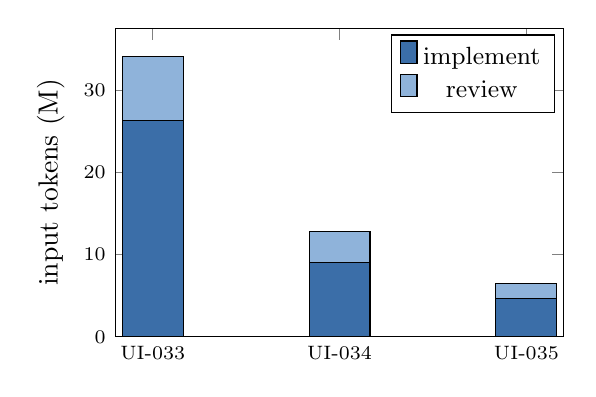
\begin{tikzpicture}
\begin{axis}[ybar stacked, bar width=22pt, width=0.6\linewidth, height=5.5cm,
  symbolic x coords={UI-033,UI-034,UI-035},
  xtick=data, ylabel={input tokens (M)}, ymin=0, legend style={at={(0.98,0.98)},anchor=north east,font=\small},
  tick label style={font=\scriptsize}]
\addplot[fill=impl] coordinates {(UI-033,26.3) (UI-034,9.0) (UI-035,4.6)};
\addplot[fill=rev] coordinates {(UI-033,7.8) (UI-034,3.8) (UI-035,1.9)};
\legend{implement, review}
\end{axis}
\end{tikzpicture}
\end{center}

Wasted: nothing thrown away. UI-033's reopen round (\$1.08 review + \$0.57 fix) bought a real
regression fix. Input is 75\% implementation, 64\% of it on UI-033, the one \texttt{hard} ticket.

\section*{Comparison with previous runs}

From \texttt{run-log.md}. The sibling \texttt{qa-input} lane: \$3.05 for 2 merged tickets (\$1.52
each), one reopen. The previous three-ticket lane, \texttt{ui-screens}: \$13.62 (\$4.54 each), two
reopened, five stages that did not reach review. The \texttt{ui-polish} lane: \$2.40 for 2, no
reopen. This run: \$5.78 for 3 (\$1.93 each), every stage-2 handoff reached review on the first
attempt. UI-033's 23-minute first implementation is the lane's longest stage; reviews cost
\$0.54--1.08 (\$0.78--1.44 in \texttt{ui-screens}).

\section*{Observations per model}

\begin{itemize}
  \item \textbf{gpt-6.1-terra xhigh, stage 2} (4 stages, 3 tickets): every handoff test-first with
        the red run recorded, captures attached for the visual tickets. It updated existing layout
        tests to virtual coordinates and named why each changed. It missed the repertoire popups
        that the ticket's ``check them all'' covered. Its ticket writes are untidy: whole
        \texttt{\#\# Comments} blocks duplicated in all three tickets (and UI-037 in the sibling
        lane), and UI-035 rewritten with a BOM and ``n\~{a}o'' double-encoded.
  \item \textbf{gpt-6.1-sol xhigh, review} (4 stages, 3--6~min): the one finding came with a
        reproduction capture, exact control rectangles and a baseline run without the stretch; its
        other reviews ran independent probes (8 scenarios on UI-034 and UI-035). It cleaned the
        duplicated blocks and the mojibake on merge. It did not comment on UI-034's inactive clock
        having no visible box in focus mode (left to Bruno, \texttt{Review: human}).
  \item \textbf{opus-5.5 xhigh, proxy}: one call, granting the two popup files and their test and
        keeping \path{ui/opening_picker.gd} out unless a red test showed it clipping; the re-review
        confirmed the picker fits.
\end{itemize}

\section*{Driver and runtime issues}

\begin{enumerate}
  \item \textbf{Self-update on a branch without upstream.} \texttt{git pull --ff-only} in
        Agent-Skills failed because the checkout was on the local \texttt{sweatshop-dashboard}
        branch; both lanes threw \texttt{Driver update failed; no runtime loaded.} before Preflight.
        The rule is deliberate (a stale driver is the bug it prevents); the message did not name
        the repository.
  \item \textbf{``local edits; not updated''.} After the switch to \texttt{main}, the untracked
        \path{sweatshop/dashboard/} folder left by that branch made the driver skip its update and
        run as is. The scripts were identical to \texttt{origin/main}, so nothing ran stale this
        time.
  \item \textbf{Ticket encoding.} Stage 2's write of UI-035 added a UTF-8 BOM and double-encoded
        Bruno's quoted ``não'' (the Windows PowerShell 5.1 \texttt{Set-Content} pattern). No
        handoff check caught it; review fixed the text but the BOM remains on the session.
  \item No crash, timeout or API error. Shutdown 1.0--1.8~s per stage. Codex reached the proxy
        directly.
  \item The new clones needed \texttt{godot --headless --import}; the import rewrote
        \path{fonts/NotoSans-Variable.ttf.import} line endings (restored by checkout), as in every
        earlier lane.
\end{enumerate}

\section*{Recommendations}

\begin{enumerate}
  \item Have the driver's update failure name the skills repository and its branch, and treat
        untracked files the way it treats a clean tree, or say which files blocked the update
        (issues 1 and 2).
  \item Add a handoff check that refuses a ticket file with a BOM or with \texttt{Ã}/\texttt{â€}
        sequences that were not in the base, or tell stage 2 in \texttt{ticket-flow} to write
        tickets as UTF-8 without BOM (issue 3).
  \item For tickets that change a global setting (stretch, theme), list the known callers in the
        ticket when it is written: a grep of \texttt{root.size} would have put the two popup files
        in Primary files and avoided UI-033's reopen and the proxy call.
  \item Lineup: keep the default Terra lineup for these UI tickets. Scoreboard rows:
        \texttt{gpt-6.1-terra xhigh $\rightarrow$ gpt-6.1-sol xhigh} 34 reviews, 38\% reopened (S2
        38\%), against \texttt{gpt-6.1-terra high} 30\% (20 reviews) and \texttt{gpt-6.1-sol high}
        23\% (22) under the same reviewer. Terra xhigh still trails both, but this run's three
        tickets cost \$1.93 each.
\end{enumerate}

\section*{Human debt and proxy decisions}

No \texttt{Débito humano:} lines in this run's tickets. One proxy call, by
\texttt{opus-5.5 xhigh} (Codex reached the proxy directly):

\begin{itemize}
  \item UI-033 (stage 2, after the reopen): \texttt{Proxy decided}: ``Yes, with one condition. Add
        \texttt{ui/repertoire\_screen.gd}, \texttt{ui/repertoire\_editor.gd} and
        \texttt{tests/test\_repertoire.gd} to Primary files now. Leave
        \texttt{ui/opening\_picker.gd} and \texttt{tests/test\_catalog.gd} out unless a red test
        shows the picker clipping. The P1 is a regression caused by this ticket's own stretch
        change, and the fix is two lines with no change to any interface.''
\end{itemize}

\section*{Acceptance}

Feature goal (Bruno's QA items 1--3 and 8): the UI looks the same windowed and fullscreen, the
board is centred, focus mode shows only board and clocks, and a finished game always has a way out.
Probes on the session head \texttt{b52737c}: the foreman captured RepertoireEditor, Repertoire and
Review at 1920$\times$1080 with \path{scripts/screens.gd} into
\path{%TEMP%/qa-layout-accept/}: the editor fits the canvas with Cancel and Save visible (UI-033's
P1 fixed), Repertoire and Review show no clipped control. Reused evidence for identical code:
UI-033's geometry probes (same 1422$\times$800 canvas and board centre 711 at all three 16:9 sizes,
grip resizing with the centre kept), stage 2's Home and Game captures at 720p/1080p/1440p, the
foreman's comparison of UI-034's focus capture with \path{focus-reference.png} (placement matches;
the inactive clock has no visible box), UI-034 and UI-035's 8-scenario review probes. Gate on the
final ticket: 493 passed, 0 failed (6 live-Lc0 checks and 1 graphical check skipped). Not examined:
real fullscreen on hardware, a live 1+0 game in focus mode, losing on time and leaving through New
game, and Bruno's visual judgement of the centred layout.

\section*{Reopen attribution}

Labelled by the foreman (opus-5.5); the reviewer was \texttt{gpt-6.1-sol xhigh}, so no
self-judging. Row appended to \path{.scratch/reopen-attribution.md}.

{\small\noindent
\begin{tabularx}{\linewidth}{@{}>{\raggedright\arraybackslash}p{1.7cm}X>{\raggedright\arraybackslash}p{2.7cm}X@{}}
\toprule
Ticket (round) & Finding & Label & Why \\
\midrule
UI-033 (1) & Repertoire popups sized from physical \texttt{root.size}; Save/Cancel off-canvas at 1080p & S2-explícito/\allowbreak código & item 1: every size that assumed window pixels now sees virtual pixels, ``check them all''; the scope call was the proxy's, the fix needed only care \\
\bottomrule
\end{tabularx}
}

Totals, reopens: S2-explícito/código 1; fixed in review: none (the merging reviews authored no
behaviour or proof). No review-induced churn, no drip-feed. The sibling \texttt{qa-input} lane
recorded UI-037 round 1 (resize-grip corner, S2-explícito/código, borderline) in PR \#39.

\section*{Scoreboard}

\texttt{scoreboard.ps1} over the ClassyCall, EasyMath, P-Chess, PhysiSyst, SIGAA-ME and SynchroNice
main checkouts (P-Chess's main checkout holds both QA lanes' rows and attribution after the
copy-back). Moved since the \texttt{ui-screens} report (the \texttt{ui-review}, \texttt{ui-polish}
and both QA lanes ran in between): implementer \texttt{gpt-6.1-terra xhigh} 27 $\to$ 43 stage runs,
5 $\to$ 7 failed; pair \texttt{gpt-6.1-terra xhigh} $\rightarrow$ \texttt{gpt-6.1-sol xhigh} 20
$\to$ 34 reviews, 40\% $\to$ 38\% reopened (S2 38\%), fixed in review for S2 2 $\to$ 3. Other pairs
under the same reviewer unchanged. Interventions: human-rescue 31 $\to$ 32 (the Agent-Skills
branch), automatic-recovery 112 $\to$ 114, proxy-decision (opus-5.5 xhigh) 15 $\to$ 19.

{\tiny
\begin{verbatim}
| Implementer | Stage runs | To review | Failed | Asked | Median min to review | Cost |
|---|---|---|---|---|---|---|
| gpt-6.1-sol high | 68 | 63 | 0 | 5 | 9m | $47.66 (68/68 priced) |
| opus-5.5 xhigh | 18 | 14 | 4 | 0 | 12m | $91.78 (18/18 priced) |
| gpt-6.1-sol max | 6 | 5 | 0 | 1 | 24m | $12.12 (6/6 priced) |
| opus-5.5 high | 20 | 13 | 6 | 1 | 6m | $37.46 (20/20 priced) |
| gpt-6.1-sol xhigh | 10 | 10 | 0 | 0 | 12m | $7.57 (10/10 priced) |
| gpt-6.1-terra high | 32 | 20 | 10 | 2 | 7m | $8.54 (32/32 priced) |
| gpt-6.1-terra xhigh | 43 | 35 | 7 | 1 | 9m | $31.24 (43/43 priced) |
(rows for older models unchanged since the ui-screens report)

| Implementer | Reviewer | Reviews | Reopened | Reopen rate | Reopened for S2 | S2 rate | Unclassified | Fixed in review for S2 |
|---|---|---|---|---|---|---|---|---|
| gpt-6.1-sol high | gpt-6.1-sol max | 38 | 12 | 32% | 9 | >=24% | 2 | 1 |
| gpt-6.1-sol high | gpt-6.1-sol xhigh | 22 | 5 | 23% | 5 | 23% | 0 | 0 |
| gpt-6.1-sol xhigh | gpt-6.1-sol xhigh | 10 | 1 | 10% | 1 | 10% | 0 | 1 |
| gpt-6.1-terra high | gpt-6.1-sol xhigh | 20 | 6 | 30% | 6 | 30% | 0 | 0 |
| ? | gpt-6.1-sol xhigh | 4 | 1 | 25% | 0 | 0% | 0 | 0 |
| gpt-6.1-terra xhigh | gpt-6.1-sol xhigh | 34 | 13 | 38% | 13 | 38% | 0 | 3 |
(other pairs unchanged since the ui-screens report)

| Implementer -> Reviewer | Rounds | S2 explicit code | S2 explicit test | S2 implicit | S1 | S3 noise |
|---|---|---|---|---|---|---|
| gpt-6.1-terra high -> gpt-6.1-sol xhigh | 9 | 10 | 1 | 3 | 1 | 0 |
| gpt-6.1-terra xhigh -> gpt-6.1-sol xhigh | 16 | 18 | 0 | 8 | 3 | 0 |

| Discovery | Recorded findings | Earlier review miss (yes / known) | Review-induced churn (yes / known) |
|---|---|---|---|
| ticket-review | 409 | 7 / 214 | 1 / 216 |
| session-review | 32 | 25 / 27 | 0 / 31 |
| release-audit | 2 | 2 / 2 | 0 / 2 |
Runtime completion to process exit: 403.749s total over 317 measured stages; 334 unmeasured.
| Intervention | Recorded events |
|---|---|
| human-rescue | 32 |
| automatic-recovery | 114 |
| proxy-decision (unknown) | 37 |
| routine-approval | 18 |
| proxy-decision (gpt-6-astra high, fallback) | 58 |
| proxy-decision (opus) | 42 |
| proxy-decision (supervisor) | 12 |
| proxy-decision (opus-5.5 xhigh) | 19 |
\end{verbatim}
}

With 34 reviews the Terra xhigh pair is past the anecdote line; the Terra high and Sol high pairs
it is compared with have 20 and 22.

\section*{Pending for the human}

\begin{enumerate}
  \item Review PR \#40 (two \texttt{Review: human} tickets): judge
        \path{%TEMP%/pchess-ui033/} (Home and Game at 720p/1080p/1440p, armed Resign at 800 and
        600) and \path{%TEMP%/pchess-ui034-capture/focus-final.png}; decide whether the inactive
        clock in focus mode needs a box.
  \item By hand: Home and a 3+2 game in a 1280$\times$720 window, then fullscreen; a 1+0 game in
        focus mode (F11, Esc Esc, game-over card, F11 back); lose a 1+0 on time, close the card with
        X, press New game.
  \item After merging PR \#40 or PR \#39, tell the other lane's foreman to sync.
\end{enumerate}

\end{document}
